The goal of our end-to-end evaluation is to understand how the cluster file
system scales with multiple metadata servers.
As shown in Table \ref{tab:setting}, PanFS consists of five shelves; in other
words, PanFS has a total of five metadata servers (called director blades) and
fifty object servers (called OSD blades).
Ideally, a \sys server should be co-located with the metadata server; such a
setup will allow the cluster file system to scale metadata performance as more
\sys servers and metadata servers are added.
However, this would require a few configuration changes to allow \sys server
process to run on the PanFS metadata servers. 

Because our goal is to avoid any configuration changes, we used five additional
test nodes, each with 64 cores and a 40 GigE NIC, that together can saturate 
the 5-shelf PanFS storage cluster.
Each test node has three subsystems: one \sys server, 32 \sys clients and a 
PanFS DirectFlow (client) module.  
Each \sys client is a library that is linked with a workload generating
application. These clients send file operations to the \sys servers. The \sys
server stores and accesses file system metadata through the PanFS DirectFlow
module. In addition, the \sys clients can also communicate with the cluster
file system through the PanFS DirectFlow module (this path is used to access
the file data as described in earlier sections).
In the rest of this section, this layering of \sys on PanFS is called \psys.
In summary, the \psys configuration consists of a total of 160 workload 
generating application threads (linked with 160 \sys clients) that communicate 
with 5 \sys servers that use the 5 metadata servers in the underlying PanFS 
storage cluster. 

To generate application workloads, we use two HPC benchmarks that are used
widely by vendors and users of parallel file systems. 
To test the metadata path, we used the \textit{mdtest} synthetic benchmark 
\cite{mdtest}.
To test the data path, we used LANL's File System Test Suite checkpoint 
benchmark\cite{mpiio}.

\textbf{Metadata Intensive Workloads -- }
We use the synthetic {\it mdtest} benchmark to generate a three-phase workload:
The first phase creates 5 million
zero-files in a single shared directory \cite{ceph:weil06, GIGA11}.
The second phase performs $stat()$ on random files in this large directory.
The third phase deletes all files in this directory in a random order.
%Each phase uses all the 160 clients to issue operations concurrently in a
%random order.

We compare the performance of native PanFS and \psys for this benchmark.
However, to ensure a fair comparison we cannot compare them directly. This is
because of two reasons: first, a single directory can only utilize one PanFS 
metadata server, and second, PanFS directories can contain at most 1 million 
files.
For a fair comparison, we compare \psys with native PanFS that creates 1 million 
files in 5 different directories owned by 5 different metadata servers.

\begin{figure}[t]  %%%%%%%%%%%%%%%%%%%%%%%
\centerline{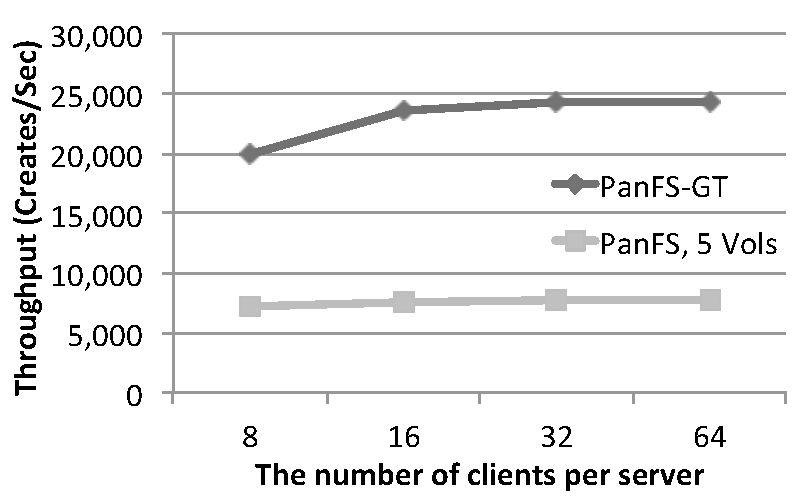
\includegraphics[scale=0.7]{./figs/zero_file_creation_on_panfs}}
\vspace{10pt}
\caption{
\textit{Average throughput during creating five million zero-length files
in one empty directory with different number of clients per test node.
Running 32 and more clients per test node is able to saturate \psys
and original PanFS}
}
%\vspace{10pt}
\hrule
\label{graph:creation_clients}
\end{figure}       %%%%%%%%%%%%%%%%%%%%%%%

\begin{figure}[t]  %%%%%%%%%%%%%%%%%%%%%%%
\centerline{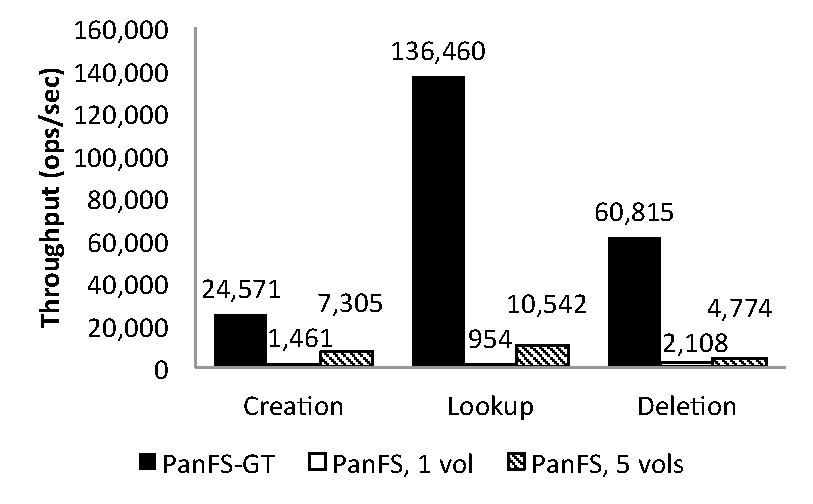
\includegraphics[scale=0.7]{./figs/mdtest}}
\vspace{10pt}
\caption{
\textit{
The average aggregated throughput of different operations in {\it mdtest}
when generating 5 million zero-length files in a single shared directory.
Since PanFS has a hard limit to allow only create 1 million entries
in one directory, the bar showing PanFS with 1 volume only gives
the average throughput for the case of creating 1 million entries.
}
}
%\vspace{10pt}
\hrule
\label{graph:mdtest_ops}
\end{figure}       %%%%%%%%%%%%%%%%%%%%%%%

Figure \ref{graph:creation_clients} shows the aggregated throughput during
the first phase. We vary the number of clients running in each test node
to determine the number of clients needed to saturate both \psys and native
PanFS systems.
Both systems achieve the highest aggregated throughput using 32 or more number 
of clients per node. In all the experiments shown later, by default, we report 
results with 32 clients per test node.
For all cases, \psys is approximately 3.5 times faster than the native PanFS
using 5 volumes. The aggregated peak throughput for the 5-server and
160-client system is about 25,000 file creates per second. 

Figure \ref{graph:mdtest_ops} shows the aggregated throughput of
different operations during the three-phase {\it mdtest} workload.
In addition to the \psys and 5-shelf PanFS, this figure also reports the 
aggregated throughput of creating 1 million files in single-shelf PanFS.
For $lookup$ and $deletion$ workloads, \psys outperforms native PanFS by a
factor to 10 to 15 higher operations per second.
Fast lookup performance results from memory indexing and Bloom filters in \ldb.
For deletion of a key, \ldb essentially just inserts a new entry with the 
deletion mark next to the key to be deleted, and delays the actual deletion in 
later compaction processes.


\textbf{Small File Workloads -- }
We also use {\it mdtest} benchmark to generate small file workloads to evaluate
the effectiveness of embedding file content with the metadata inside \tfs.
In this test, {\it mdtest} benchmark creates 5 million files in 
a single directory, and writes 4KB and 16 KB of data in these files. Our choice
of file sizes is motivated by prior file system studies that have observed
that 4KB is the median file size for many desktop workloads \cite{Bill11}
and 16KB is the median file size for large PanFS storage clusters \cite{brent13}.
The threshold for embedding files, $T$, for our prototype is set to 64KB, so all 
these files are stored in \tfs instance.

%compaction and CPU usage
Figure \ref{graph:smallfiles} shows the aggregated throughput of both \psys and
native PanFS during the small file workload test.
We observe that \psys is about $2.5\times$ faster than native PanFS for 4KB
files.
However, \psys is about $35\%$ slower than PanFS for 16KB file size.
We found that embedding 16KB file makes the key-value pair significantly larger.
This causes higher write amplification during \ldb compactions because
\ldb compactions will try to merge-sort both file data and metadata.
Additionally, \ldb writes the inserted key-value pairs twice: first
to the transaction log and then (during a compaction) to the SSTable.
With larger key-value pairs, LevelDB's per-operation efficiency is reduced due
to the increased cost of extra copies of large values.
This suggests that the threshold $T$ for embedding file size should not be
greater than 16KB. Embedding larger files may sacrifice read performance for
faster insertion rate; this may be done using a column-oriented layout approach 
that stores metadata and small file separately.
These tradeoffs are not studied in this paper and left for future work.

\begin{figure}[t]  %%%%%%%%%%%%%%%%%%%%%%%
\centerline{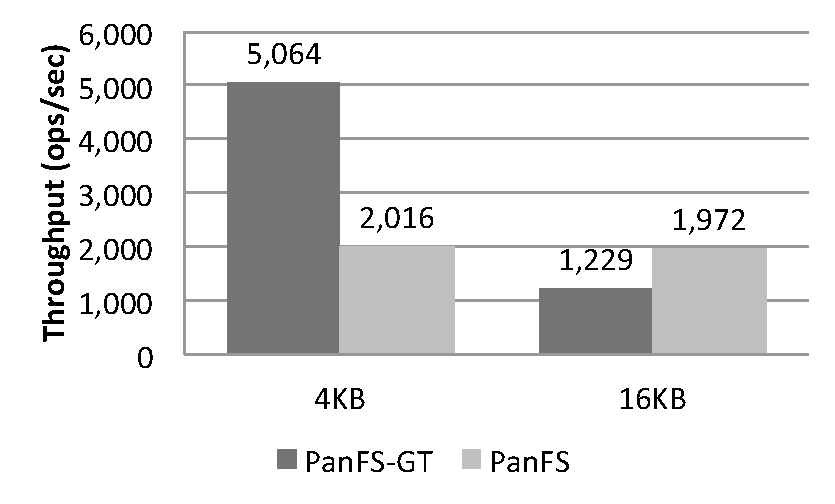
\includegraphics[scale=0.7]{./figs/small_file_creates}}
\vspace{10pt}
\caption{
\textit{Average aggregated throughput during creating 5 million small files
with different size in one shared directory}
}
%\vspace{10pt}
\hrule
\label{graph:smallfiles}
\end{figure}       %%%%%%%%%%%%%%%%%%%%%%%


%Library version not FUSE
%Clean cache

\textbf{Data Intensive Workloads -- }
To study the data path throughput, we use the LANL filesystem checkpoint 
benchmark to generate different types for HPC checkpoint I/O patterns
\cite{mpiio}.
Our experiments use this benchmarking tool to generate a concurrent N-
N checkpoint write and read workload.

All checkpoint I/O is performed by a set of processes
that synchronize with each other using MPI barriers.
At the beginning, each process creates and opens a new checkpoint file
for writing. 
Each process then waits at a barrier until all processes are ready to write.
Once all processes are ready, each process starts to write the checkpoint data 
to its own file (and all processes do this writing concurrently).
Once a process has written the specified number of bytes, it waits for all
other processes to finish writing, and then syncs its data to the file system
before closing the file.
Before starting the read phase, we terminate all processes
accessing these checkpoint files so that
we can unmount the filesystem in order to ensure that
all freshly written data has been flushed out from all the nodes' memory
to prevent any performance side-effects from caching.
After the filesystem has been mounted again,
the benchmark reads the checkpoint in the same way it was written,
however we shift, so each process will read
the file generated by another process.

In this test, we also vary the number of clients per test node
from 8 to 64 clients. The clients in each node will generate a total of
640GB checkpoint data to the underlying file system.
The size of data buffer for each file system call is set to be 16KB.
For \psys, the checkpoint files generated in the test will be
first stored in \tfs, and then migrated to the underlying PanFS.

Figure \ref{graph:checkpoint_write} and \ref{graph:checkpoint_read}
show the average throughput during the write phase and read phase
in the N-N checkpoint workload respectively. 
For the checkpoint writing case, in Figure \ref{graph:checkpoint_write}, we 
observe that \psys write throughput is comparable with the native PanFS. In
fact, for smaller configurations with 8 clients per server, \psys outperforms
native PanFS by about 20\%.
For the checkpoint reading workload, in Figure \ref{graph:checkpoint_read}, 
\psys reads about 10\% slower than native PanFS.

\begin{figure}[t]  %%%%%%%%%%%%%%%%%%%%%%%
\centerline{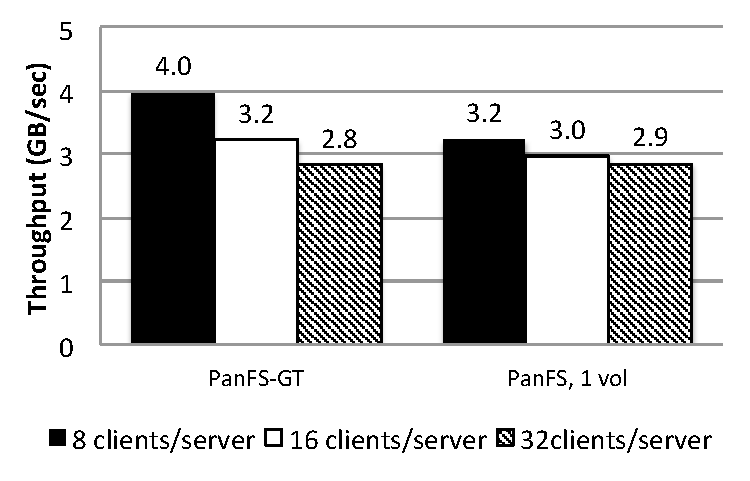
\includegraphics[scale=0.7]{./figs/checkpointing_write}}
\vspace{10pt}
\caption{
\textit{
The aggregated write throughput in N-N check-pointing workload.
Each volume receives 640 GB data.
}
}
%\vspace{10pt}
\hrule
\label{graph:checkpoint_write}
\end{figure}       %%%%%%%%%%%%%%%%%%%%%%%

\begin{figure}[t]  %%%%%%%%%%%%%%%%%%%%%%%
\centerline{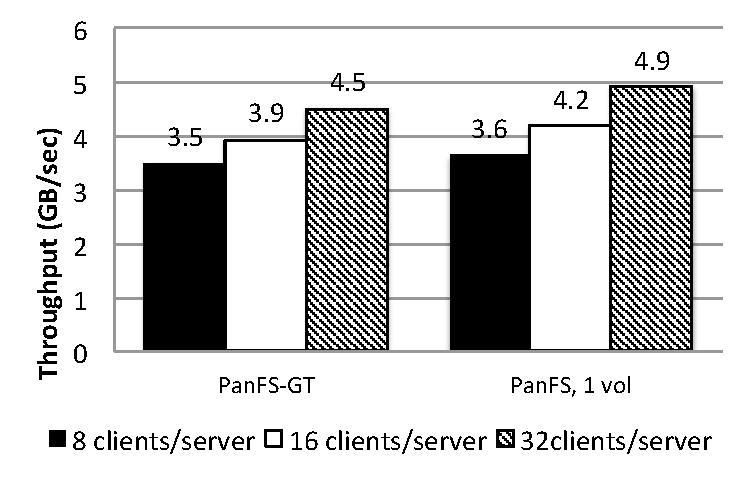
\includegraphics[scale=0.7]{./figs/checkpointing_read}}
\vspace{10pt}
\caption{
\textit{
The aggregated read throughput in N-N check-pointing workload.
}
}
%\vspace{10pt}
\hrule
\label{graph:checkpoint_read}
\end{figure}       %%%%%%%%%%%%%%%%%%%%%%%

